% arara: latexmk: { options: [ '-pdf' ] }
% arara: latexmk: { options: ['-c' ] }
\documentclass{article}

\title{Physics C Unit 7 FRQs}
\author{Henry Beveridge}
\date{\today}
\usepackage{amsmath}
\usepackage{tikz}

\begin{document}

\maketitle

\pagebreak

\section{FRQ 1}

\subsection{Part A}

\subsubsection{Part i}

For a physical pendulum, the period of oscillation is given by the formula
$$
T = \frac{2\pi}{\omega} = \frac{2\pi}{\sqrt{\frac{mgd}{I}}} = 2\pi\sqrt{\frac{I}{mgd}}
$$
where $I$ is the moment of inertia of the pendulum, $m$ is the mass of the pendulum, $g$ is the acceleration due to gravity, and $d$ is the distance from the pivot point to the center of mass of the pendulum.

Thus, we first need to derive a formula for $I$ and $d$ in terms of the given variables ($M$, $\lambda$, and $H$).

For $I$,
$$
I = \int_0^H dm r^2 = \int_0^H \lambda y^2 dy = c \int_0^H y^3 dy = c \frac{H^4}{4}
$$


For $d$, we need to find the center of mass of the pendulum.
$$
y_{com} = \frac{\int y dm}{M} = \frac{\int_0^H y \lambda dy}{M} = \frac{\int_0^H cy^2 dy}{M} = \frac{cH^3}{3M}
$$

Substituting these into the formula for $T$,
$$
T = 2\pi\sqrt{\frac{I}{mgd}} = 2\pi\sqrt{\frac{c\frac{H^4}{4}}{Mg\frac{cH^3}{3M}}} = 2\pi\sqrt{\frac{3H}{4g}}
$$


\subsubsection{Part ii}

% The change in oscillation period depends on both $I$ and $d$ because they are the only variables changing between these two objects. Thus, we must compute $I$ and $d$ for this new object.
%
% Since the shape of the two objects are the same, the $I_{2}$ about the original pivot is simply $I_1$ with $2H$ in place of $H$.
% $$
% $$
% $I_{2,com}$ can be found using the parallel axis theorem, again with $2H$ in place of $H$.
% $$
% I_{2,com} = I_{2,pivot} - Md^2 = 16\frac{cH^4}{4} - MD^2
The key thing to note is that $D$, the distance between the COM and the pivot point is constant between the two objects. So,

So, the only thing that matters is the moment of inertia of the two objects. We know that because the mass remains constant but the total distance increases, the moment of inertia of the second object must be greater.

$$
d_1=d_2, I_1 < I_2 \implies T_1 < T_2
$$


\subsection{Part B}

First, note that $I_{2,com}$ is basically the same as $I_{1,com}$ except 4 times as great because distances are squared in the moment of inertia defenition. Finding $I_{1,com}$:
$$
I_{1,com} = I_{1,pivot} - MD^2
$$

Finding $I_{2,com}$:

$$
I_{2,com} = 4 I_{1,com} = 4(I_{1,pivot} - MD^2) = 4I_{1,pivot} - 4MD^2
$$

Finding $I_{2,pivot}$:

$$
I_{2,pivot} = I_{2,com} + MD^2 = 4I_{1,pivot} - 3MD^2
$$

\section {FRQ 2}

\subsection {Part A}

The key thing to note here is that they're looking for $\frac{T}{2}\le t \le T$, so that can throw you off.

\vspace{0.4cm}

\begin{center}
  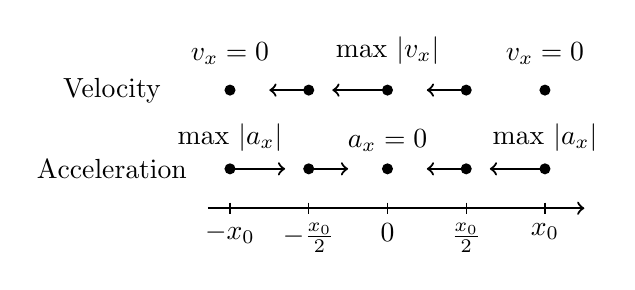
\begin{tikzpicture}
    \fill (0,0.5) circle (2pt);
    \fill (1,0.5) circle (2pt);
    \fill (2,0.5) circle (2pt);
    \fill (3,0.5) circle (2pt);
    \fill (4,0.5) circle (2pt);
    \fill (0,1.5) circle (2pt);
    \fill (1,1.5) circle (2pt);
    \fill (2,1.5) circle (2pt);
    \fill (3,1.5) circle (2pt);
    \fill (4,1.5) circle (2pt);
    \draw[thick,->] (-8pt,0) -- (4.5 cm,0);
    \draw (0,2pt) -- (0,-2pt) node[anchor=north] {$-x_0$};
    \draw (1,2pt) -- (1,-2pt) node[anchor=north] {$-\frac{x_0}{2}$};
    \draw (2,2pt) -- (2,-2pt) node[anchor=north] {$0$};
    \draw (3,2pt) -- (3,-2pt) node[anchor=north] {$\frac{x_0}{2}$};
    \draw (4,2pt) -- (4,-2pt) node[anchor=north] {$x_0$};
    \node[] at (-1.5,0.5) {Acceleration};
    \node[] at (-1.5,1.5) {Velocity};
    
    \node[anchor=south] at (0,1.7) {$v_x=0$};
    \node[anchor=south] at (4,1.7) {$v_x=0$};
    \draw[thick,->] (1,1.5) -- (0.5,1.5);
    \draw[thick,->] (2,1.5) -- (1.3,1.5);
    \node[anchor=south] at (2,1.7) {max $|v_x|$};
    \draw[thick,->] (3,1.5) -- (2.5,1.5);

    \node[anchor=south] at (2,0.6) {$a_x=0$};
    \draw[thick,->] (0,0.5) -- (0.7,0.5);
    \node[anchor=south] at (0,0.6) {max $|a_x|$};
    \node[anchor=south] at (4,0.6) {max $|a_x|$};
    \draw[thick,->] (1,0.5) -- (1.5,0.5);
    \draw[thick,->] (3,0.5) -- (2.5,0.5);
    \draw[thick,->] (4,0.5) -- (3.3,0.5);


  \end{tikzpicture}
\end{center}

\subsection {Part B}

Max potential energy = max kinetic energy, so just solve those equations.

$$
U_{max}=K_{max}
$$
$$
mgh=\frac{1}{2}m v_{max}^2 \implies v_{max}=\sqrt{2gh}
$$
$$
v_{max}=\sqrt{2gh}=\sqrt{2gBx_0^2}=x_0\sqrt{2gB}
$$

\subsection {Part C}

Now we're back to the interval $0\le t\le T$.

\begin{center}
  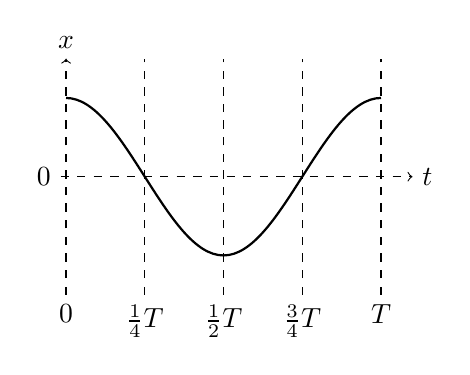
\begin{tikzpicture}
    \draw[dashed,->] (-2pt,0) node[anchor=east] {$0$} -- (4.4cm,0) node[anchor=west] {$t$};
    \draw[dashed,->] (0,-1.5) node[anchor=north] {$0$} -- (0,1.5) node[anchor=south] {$x$};
    \draw[dashed] (1,-1.5) node[anchor=north] {$\frac{1}{4}T$} -- (1,1.5);
    \draw[dashed] (2,-1.5) node[anchor=north] {$\frac{1}{2}T$} -- (2,1.5);
    \draw[dashed] (3,-1.5) node[anchor=north] {$\frac{3}{4}T$} -- (3,1.5);
    \draw[dashed] (4,-1.5) node[anchor=north] {$T$} -- (4,1.5);

    \draw[thick] (0,1) cos (1,0) sin (2,-1) cos (3,0) sin (4,1); 
  \end{tikzpicture}
\end{center}


\begin{center}
  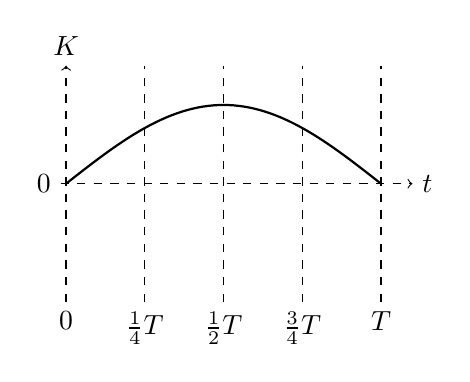
\begin{tikzpicture}
    \draw[dashed,->] (-2pt,0) node[anchor=east] {$0$} -- (4.4cm,0) node[anchor=west] {$t$};
    \draw[dashed,->] (0,-1.5) node[anchor=north] {$0$} -- (0,1.5) node[anchor=south] {$K$};
    \draw[dashed] (1,-1.5) node[anchor=north] {$\frac{1}{4}T$} -- (1,1.5);
    \draw[dashed] (2,-1.5) node[anchor=north] {$\frac{1}{2}T$} -- (2,1.5);
    \draw[dashed] (3,-1.5) node[anchor=north] {$\frac{3}{4}T$} -- (3,1.5);
    \draw[dashed] (4,-1.5) node[anchor=north] {$T$} -- (4,1.5);

    \draw[thick] (0,0) sin (2,1) cos (4,0);
  \end{tikzpicture}
\end{center}

\subsection {Part D}

In the formula for $v_{max}$ derived in Part B, $x_0$ is only to the first power, so the ratio would simply be $2:1$. This is checked pretty easily because twice the $x$ means four times the height, which means four times the potential energy. This means max kinetic energy is four times as much, and because $v$ is squared in kinetic energy, the resultant factor is simply $2$.

\section {FRQ 3}

\subsection {Part A}

For each spring with a known spring constant, attach the rock to the spring, and compress the spring any distance. Then, time how long it takes the spring compress and extend 50 times. Record this time and the spring constant. Do this 10 times for each spring, and average the time result.

\subsection {Part B}

Take the time it takes for 50 compression/extensions and divide by 50 to get the period. Then, plot $\frac{1}{k}$ on the x-axis and plot $(\frac{2pi}{T})^2$ on the y-axis. The slope of the best line of fit will be approximately equal to $m$.

\subsection {Part C}

\subsubsection {Part i}

A relationship between $L_s$ and $t_{10}$ can be obtained by using the equation for period of a pendulum. Note for a linear relationship, $L_s$ must be square rooted.
$$
T = 2\pi\sqrt{\frac{L}{g}}
$$

Horizontal Axis: $\sqrt{L_s}$

Vertical Axis: $t_1$

\begin{center}
  \begin{tabular}{|c|c|}
    \hline
    Time for 1 oscillation (s) & $\sqrt{L_s}$ $(m^\frac{1}{2})$\\
    \hline
    2.72 & 0.693 \\
    \hline
    2.41 & 0.592 \\
    \hline
    1.83 & 0.447 \\
    \hline
    1.33 & 0.316 \\
    \hline
    1.01 & 0.224 \\
    \hline
  \end{tabular}
\end{center}

\subsubsection {Part ii}

\begin{center}
  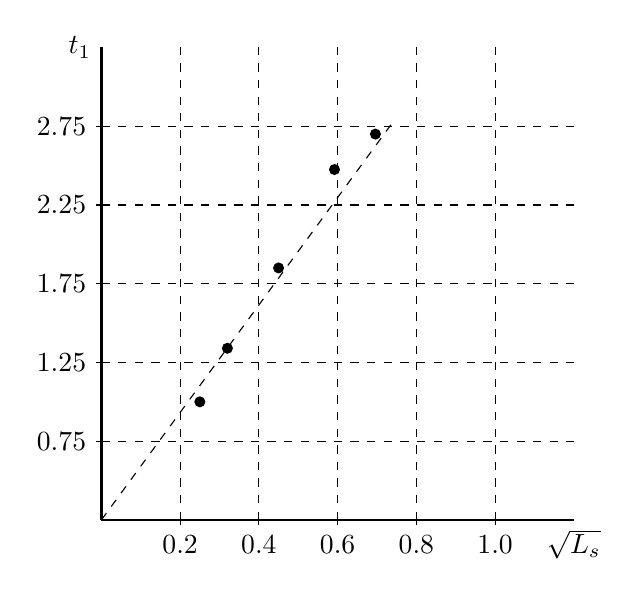
\begin{tikzpicture}
    \draw[thick] (0,0) -- (0,6) node[anchor=east] {$t_1$};
    \draw[thick] (0,0) -- (6,0) node[anchor=north] {$\sqrt{L_s}$};
    \draw (1,-2pt) node[anchor=north] {$0.2$} -- (1,2pt); 
    \draw (2,-2pt) node[anchor=north] {$0.4$} -- (2,2pt); 
    \draw (3,-2pt) node[anchor=north] {$0.6$} -- (3,2pt); 
    \draw (4,-2pt) node[anchor=north] {$0.8$} -- (4,2pt); 
    \draw (5,-2pt) node[anchor=north] {$1.0$} -- (5,2pt); 
    \draw (-2pt,1) node[anchor=east] {$0.75$} -- (2pt,1); 
    \draw (-2pt,2) node[anchor=east] {$1.25$} -- (2pt,2); 
    \draw (-2pt,3) node[anchor=east] {$1.75$} -- (2pt,3); 
    \draw (-2pt,4) node[anchor=east] {$2.25$} -- (2pt,4); 
    \draw (-2pt,5) node[anchor=east] {$2.75$} -- (2pt,5); 

    \foreach \x in {1,2,3,4,5}
    {\draw[dashed] (\x,0) -- (\x, 6);
    \draw[dashed] (0,\x) -- (6, \x);}

    \fill (3.48,4.9) circle (2pt);
    \fill (2.96, 4.45) circle (2pt);
    \fill (2.25, 3.2) circle (2pt);
    \fill (1.6, 2.18) circle (2pt);
    \fill (1.25, 1.5) circle (2pt);

    \draw[dashed] (0, 0) -- (3.7, 5.05);

  \end{tikzpicture}
\end{center}

\subsection {Part D}

Approximate the best line of fit with a slope of:
$$
\frac{2.25-1.25}{0.6-0.3} = 3.333
$$

$$
3.333 = \frac{T}{\sqrt{L}} = \frac{2\pi\sqrt{\frac{L}{g}}}{\sqrt{L}} = \frac{2\pi}{\sqrt{g}} \implies (\frac{2\pi}{3.333})^2 = g
$$

$$
g \approx 3.554 \frac{m}{s^2}
$$
\end{document}


